\chapter{Contexte du sujet}
\label{chap:contexte}
%%\begin{itemize}
	%%\item Expliquer le projet
	Notre projet est de produire une sonde qui renifle (ou sniffe) le trafic réseau dans le contexte de l'Internet des Objets. Cette sonde est un nœud dans ce réseau, et a pour but de transmettre des informations utiles à sa sécurisation et dans une certaine mesure à l'analyse de ces informations.
%%\end{itemize}

\section{Analyse de l'existant}
	
	\subsection{Internet des objets}
		%%\begin{itemize}
			%%\item Qu'est-ce que c'est ?
		L'Internet des Objets, ou Internet of Things en anglais, correspond à l'extension d'internet aux éléments ou lieux du monde physique, là où l'internet habituel s'arrête au domaine du virtuel.
		Cette technologie est implantée dans notre société avec diverses applications comme la domotique, le médical, la gestion des déchets, mais pas limité à ceux là.
		Notre projet s'inscrit donc dans cet univers puisque les sondes surveillent le trafic de différents éléments d'un sous-réseau d'objets physiques, d'un bâtiment par exemple. \\
		L'Internet des objets regroupe différents modes de communications entre les nœuds d'un réseau tels que le Wi-Fi, le courant porteur ou le bluetooth.%%\\
			%%\item Technologies utilisables (bluetooth, wifi, 6lowpan)
			%%Détailler les différentes technologies
		%%\end{itemize}
		
	\subsection{Technologies de communication}
%		\begin{itemize}
%			\item 6lowpan qu'est-ce que c'est ?
%			\begin{itemize}
%				\item définition
		6LoWPAN est une spécification du principe des LoWPAN, c'est à dire un ensemble d'équipements aux ressources limitées, puissance, autonomie entre autres, reliés dans un réseau au débit limité. Typiquement, ces réseaux sont constitués d'un grand nombre d'éléments ou nœuds dans le réseau.
		Basé sur l'IPv6, quelques problèmes se posent avec la spécification standard de celui ci. Ce protocole de communication possède une taille d'entête importante, couplée aux contraintes de tailles de paquets imposées, cela pose des soucis de fragmentation et de réassamblage excessif pour des contrôleurs aux capacités limitées.\\
%				\item exemples (Linky, domotique, industrie)
		La spécification de 6LoWPAN et ses RFC (4919 et 4944) définissent donc des solutions à ces problèmes, et on peut aujourd'hui utiliser plusieurs implémentations de 6LoWPAN, tel que ZigBee. Linky, le nouveau compteur communicant d'ERDF utilise cette technologie. Bien sûr, on peut trouver pléthore de projets et d'objets de domotique se servant de la spécification et de ses implémentations pour communiquer.
		
%			\end{itemize}
%		\end{itemize}
		
	\subsection{Sécurité des communications}
	%		\begin{itemize}
	%			\item Sécurité dans 6lowpan
	%			\begin{itemize}
	%				\item RFC définissent sécurité
		Les différentes RFC (Request For Comment) définissent un ensemble de consignes sur l'implémentation de la sécurité des réseaux 6LoWPAN notamment sur les différentes couches de la pile protocolaire.
		
		\begin{figure}[htp]
			\centering
			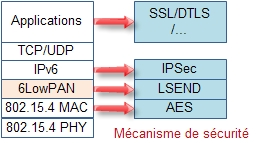
\includegraphics[width=10cm]{images/6lowpan-secu.jpg}
			\caption{Diagramme d'explication de la sécurité des couches de 6LoWPAN.}
			\label{fig:diagramme-6lowpan-secu}
		\end{figure}
		
		\begin{itemize}
			\item Sur la couche MAC : l'algorithme AES (Advanced Encryption Standard) doit être utilisé pour sécuriser la couche liaison.
			\item Sur la couche réseau : l'utilisation d'IPsec (Internet Protocol Security) est possible, mais coûteuse et un échange de clés habituel pour le chiffrement n'est pas possible. Une extension du protocole SEND -- \emph{\textbf{SE}cure \textbf{N}eighbor \textbf{D}iscovery protocol} -- (RFC 3971) permettant de sécuriser ce mécanisme a été mis en place pour les réseaux 6LoWPAN, appelé LSEND -- \emph{\textbf{L}ightweight \textbf{SE}cure \textbf{N}eighbor \textbf{D}iscovery protocol} --.
			\item Sur la couche application : une solution possible est de mettre en place la sécurisation via SSL.
		\end{itemize}
%				\item Dans les faits, pas vraiment mis en place
		
		Dans les faits, la sécurité étant difficile à mettre en place à cause des contraintes de l'embarqué (performance, stockage des données), elle est parfois insuffisante pour garantir un échange de données sécurisées.
%			\end{itemize}
%		\end{itemize}



\section{Objectif du projet}

	\subsection{Détail du projet}
		%%\begin{itemize}
			%%\item Quels types de données sont analysées ?
		Nous avons expliqué l'intitulé du projet mais non pourquoi ces sondes pouvaient être utiles. Les sondes sont des noeuds, ou mote dans le vocabulaire de Contiki, qui vont sonder et analyser le trafic circulant. Les informations qu'elles récupèrent permettent la détection d'intrusions. \\
		En effet, le trafic et les paquets sont soumis à des formats spécifiques, contenant des informations qui doivent s'y conformer. Dans le cas d'écarts par rapport au format réglementaire, on se retrouve face à une anomalie, et possiblement une attaque.\\
			%%\item système contraint en puissance et en mémoire
		La difficulté de cette analyse réside autant dans les contraintes du matériel, qui est limité en puissance et en mémoire, que dans les solutions mises en places par le réseau pour pallier à ces contraintes, par exemple la compression d'entête.
		%%\end{itemize}
	\subsection{Où s'inscrit le projet ?}
		%%\begin{itemize}
		Comme illustré précédemment, l'Internet des Objets trouve son utilité dans de nombreux domaines. Certaines applications, comme l'industrie ou le médical, font circuler des données sensibles sur le réseau, et des personnes mal intentionnées pourraient causer de graves problèmes sans être détectés si le réseau n'est pas protégé.\\
		On peut retrouver d'autres exemples ayant moins de conséquences comme les hackers changeant le nombre de places des panneaux de parking par des injures. Dans cet exemple, la personne a simplement usurpé l'identité de la machine qui met à jour les places, et a envoyé des paquets falsifiés contenant ces injures grâce à un manque de sécurité sur le réseau.
			%%\item Industrie, hopitaux, mobilier urbain ( pas "simple domotique" )
		%%\end{itemize}

\section{Réponse à un besoin de l'équipe}
	
	\subsection{Focalisation sur la sécurité par 2XS}
%	\begin{itemize}
%		\item Systèmes sûrs
%		\begin{itemize}
%			\item Preuves formelles
		L'équipe de recherche 2XS se focalise sur la création de systèmes sûrs, par le biais de différents mécanismes, dont les preuves formelles de programmes, le développement de librairies, et bien d'autres projets visant à sécuriser les systèmes.\\
		%			\item Différents projets de sécurité
		%		\end{itemize}
		%		\item Qu'en est il des communications ?
		
		La problématique de la sécurité ne s'arrête pas à la frontière du système en lui-même, il communique avec d'autres. C'est là que les failles et les fuites d'informations sont les plus nombreuses, même si l'intégrité du système n'est pas en cause.\\
		L'un de leurs projets pour répondre à ce problème est Discus.
%	\end{itemize}
	
	\subsection{Discus}
	Discus est une architecture d'IDS -- Système de détection d'intrusion -- massivement distribuée, qui est configurée grâce à un DSL -- Langage dédié -- Discus-script. Le principe de Discus est d'abstraire la définition des contraintes de sécurité sur un réseau, qu'il soit ethernet, bluetooth ou Wi-Fi.\\
	Notre projet est donc directement en rapport avec celui-ci, fournissant la couche matérielle nécessaire à Discus pour analyser le réseau afin d'y appliquer ces contraintes de sécurité.
%	\begin{itemize}
%		\item IDS -- Système de détection d'intrusion
%	\end{itemize}

\section{Technologies et systèmes utilisés}
	Pour développer notre sonde renifleuse, nous avons utilisé plusieurs outils que nous allons présenter ici :
	
	\subsection{Contiki}
	Contiki est un système d'exploitation léger et flexible avec pour cible les capteurs miniatures en réseau. Ses atouts sont sa flexibilité, sa portabilité, sa faible consommation énergétique, et surtout dans notre cas, son support des protocoles IPv6 et 6LoWPAN. Il répond à une attention importante de la communauté scientifique portée aux réseaux de capteurs sans fil. Il a été créé par une équipe du centre suédois de recherche scientifique SICS.
	
	\subsection{Outils de simulations}
	Notre sonde a été créée dans un environnement de développement fourni par le site officiel de Contiki, la machine virtuelle InstantContiki3.0, en utilisant principalement pour les tests l'outil de simulation Cooja.\\
	Cooja est un simulateur de matériel pour Contiki permettant de créer virtuellement un réseau de capteurs, de les positionner à notre envie et de charger les différents programmes pour les nœuds (ou motes dans le jargon Contiki) à la volée.
	Nous avons donc passé beaucoup de temps à l'utiliser pour tester notre programme dans des situations réalistes.
	\clearpage
	\begin{figure}[htp]
		\centering
		\includegraphics[width=16cm]{images/cooja}
		\caption{Capture d'écran de Cooja.}
		\label{fig:Cooja}
	\end{figure}

	\subsection{Langage C embarqué et sa chaîne de compilation}
	La création de la sonde s'est fait sur Contiki et le programme a dû être adapté aux contraintes du matériel pour lequel il est créé. Pour cela, nous devions rendre le code le plus léger et proche du matériel, ceci s'illustre par l'absence des librairies standard du langage C, par exemple stdlib ou unistd.\\
	La compilation des programmes se fait avec des versions de GCC spécifiques aux architectures matérielles que nous utilisons.
	
	\subsection{Git}
	Git est un gestionnaire de version de projet. Celui-ci permet de synchroniser le travail de notre binôme.\\
	Nous avons choisi d'utiliser la plateforme GitHub pour accueillir notre dépôt Git, afin de faciliter l'accès à notre code.
%%% Local Variables: 
%%% mode: latex
%%% TeX-master: "isae-report-template"
%%% End: 
